% !TEX root = ../../../main/aws_chabauty.tex
\newpage
\subsection{Lecture 4}

Our setup: Let $X/\Q$ be a nice curve of genus $g \geq 2$. We know $\rank J(\Q)= g$, $\rank NJ(J)>1$, $\log: J(\Q) \otimes \Qp \ma{\sim} H^0(X_{\Qp},\Omega^1)^*$


Let $p$ be a good prime and assume $X$ has everywhere potential good reduction. We extended the diagram
	\[
	\begin{tikzcd}
	X(\Q) \arrow{d}{j} \arrow{r} & X(\Qp) \arrow{dr}{\text{it. col. int.}} \arrow{d}{j_p} \\
	H_f^1(G_T,U) \arrow{r}{\log_p} \arrow{d}{I} &  H_f^1(G_P,U) \arrow{r} \arrow{d} & U^\dr/\Fil^0 \\
	M_{\Q,f} \arrow{r} \arrow{d} & M_P \arrow{r} & M_{\text{fil},\phi} \arrow{ddl}{h_P} \\
	H_f^1(G_T,V) \times H_f^1(V^*(1)) \arrow{dr}{h} & & \\
	& \Q_p & 
	\end{tikzcd}
	\]
Construct $\tau,\tau_P$ via twisting. Then by our assumptions, we have the following:


	\begin{figure}[!ht]
	\centering
	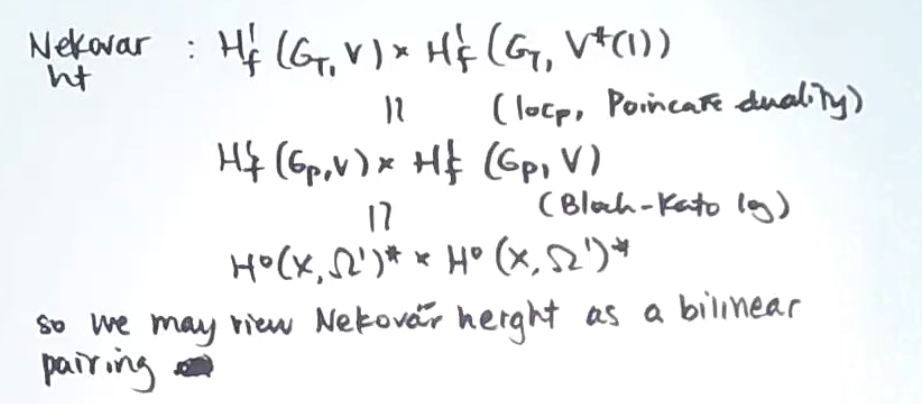
\includegraphics[width=0.5\textwidth]{../images/im46.png}
	\end{figure}


Now let $A: X(\Q) \to M_{\Q,f}$ given by $x \mapsto \tau(j(x))$, and do this similarly for $x \in X(\Qp)$. Then $x \mapsto h(\tau(j(x)))$ extends to $X(\Qp) \to \Qp$. Fix a basis $\{\psi_i\}$ of $H^0(X,\Omega^1)^* \otimes H^0(X,\Omega^1)^*$ and rewrite the height in terms of this basis using known $\Q$-points (either if enough $X(\Q)$ or $J(\Q)$). 


\begin{thm}[B-Degara]
The function $p: X(\Qp) \to \Qp$ given by $x \mapsto h_P(A(x)) - h(A(x))$ vanishes on $X(\Qp)_U$ and has finitely many zeros.
\end{thm}

To make this explicit, we need to\dots

\begin{enumerate}[1.]
\item Write $h$ in terms of a basis of $H^0(X,\Omega^1)^* \otimes H^0(X,\Omega)^*$
\item Compute $h_P \circ A$ using filtered $\phi$-module structure of $D_\cris(A(x))$.
\end{enumerate}


\begin{lem}
There exists a connection $A_Z$ with Hodge filtration and Frobenius structure such that $x^*A_z \simeq D_\cris(A(x))$. [This follows from Olsson's comparison theorem.]
\end{lem}


$A_Z$ is a unipotent isocrystal, quotient of universal 2-step unipotent connected $A_Z^\dr$ suffices to compute


\begin{enumerate}[1.]
\item Hodge filtration: defined by Hodge filtration on graded pieces and its global nature (Hadian: universal properties)
\item Frobenius structure: via Frob on $A_Z^\text{rig}$ and comparison theorem of Chanellotto-LaStrum, ? initial condition then gives a $p$-adic differential equation that we solve using Tuitman's algorithm.
\end{enumerate}


See Section 5.2 to 5.3 in the notes for more details. 


Examples of Quad. Chabauty

A problem of Diophantines (Problem 17) Book VI of Arithmetica 

Find three squares which when added give a square and such that the first one is ? square ? of the sceond and the second is the ? ?? of third. We can give positive rational $x,y$ such that
	\[
	y^2= x^8 + x^4 + x^2
	\]
Diophantus found $x= 1/2$ and $y=9/10$. Are there any others? Remove the singularity at $(0,0)$, then want $X(\Q)$ for $X: y^2= x^6+x^2+1$. $J(\Q)$ has rank 2, $J \sim E_1 \times E_2$, $\rank NS(J)=2$. Wetherell (97) determined $X(\Q)$ via covering collections and classical Chabauty-Coleman. Bianchi (19) gave a QC-solution to Diophantus' equation using $p$-adic sigma function. 
	\[
	X(\Qp)= \{\infty^\pm,(0,\pm1)(\pm1/2,\pm9/8)\}
	\]
B-Dogra (16) can apply QC to bielliptic genus 2 curves $X/K$ ($K=\Q$ or quad imag) with $\rank J(K)=2$ Computationally took $p$-adic heights on elliptic curves ?? Coleman integrals.


2. $X_0(37)(\Q(i))$: Daniels and Lozano-Robledo $X_0(37): y^2= -x^6 - 9x64 - 11x^1 + 37$ over $\Q(i)$ to (37)$X\Q(i)$ has rank 2.

B-Dogra-M\"uller: $X_0(37)(\Q(i))= \{(\pm2,\pm1),(\pm1,\pm4),\infty^\pm\}$ used QC and Mordell-Weil sieve. 

$p=41,73,101$.

$X_5(13)$, the split Cartan curve of level 13 is Bilu-Parent (91) determined Serre uniformity in split Cartan case.

Bilu-Parent-Robelledo (13) determined $X_5(l)(\Q)$ for all $l \neq 13$. 

What about $l=13$?

$g=3$ model was proved by Baran (smooth plane quartic) 

$\rank NS(J)=3$
$\rank J(\Q)=3$

B-Dogra-M\"uller Tuitman-Vonk: $\#X_S(A)(\Q)=7$ and B. $\#X_{ns}(?)(X\Q)=7$


4) $X_?(13)$: $g=3$ smooth plane quartic Banwait-Cremona Jacobian is isogeneous to $J$ of $X_S(B)$.
$\#X_{S_4}(1))(\Q)_{\text{known}}= 4$

B-Dogra-?-?-?-?-?-? ?????????

(of interest via Mazur's Probram B. last exceptional $S_4$ curve; last modular curve of level ?


5) Two other curve from Mazur's probram B

(via D.ZB)

$X_H$= $X(25)/H$, $\Gamma(25) \subset H \subset \GL_4(?)$

each has the following properties:

i. 2 known rational points
i. usual QC hypothesis satisfied 
Fit the global height pairing using the Jacobian and Coleman-Gross $p$-adic height on $J(\Q)$.

BDMTV 20 

$X_n(\Q)=2$, $X_{15}(\Q)=2$

Used QC and MWS

6) The curve $X_0(N)^+:= X_0(N)/w_N$ nice curve whose non-cupsidal points classify unordered pairs $\{E_1,E_2\}$ of elliptic curves admitting an $N$-isogeny. 

$X_0(N)^+(\Q)$ the set of cusps, CM points, exceptional points.

restrict to $N$ primes

Galbraith (96)

$g(X_0(N)^+)= 2$ iff $N \in \{67,73,103,107,167,191\}$, $g(X_0(N)^+)= 3$ iff $N \in \{97,109,113,127,139,149,151,179,239\}$ 

Y. Hasegara K. Hashimoto (96) $X_0N(N)^+$ hyperelliptic if and only if $g=2$.

So $g=3$ curves are smooth plane quartics. All satisfy the QC hypotheses:

$J:= J_0(N)^+$ has NS $\geq g$, so $\rank J(\Q)=g$.

$X_0(N)^+$ has good reduction away from N, but does not have potential good reduction on $N$. 

Can show that there's a regular semistable model of $X_1(N)^+$ over $\Z_N$ whose special fiber has unique irreducible component Best-Dagra then $h_N=0$.


Galbraight: what are the exceptional points on $X_0(N)^+$ for all such that curves of genus $ \leq 5$?


B-Best-Bianchi-Lawrence-M\"uller-T?-Vonk

$X_0(67)^+(\Q)$ $h_0$ exceptional points

$X_0(73)^+(\Q)$, $X_0(103)^+(\Q)$: 1 exceptional point up to hyperelliptic ?

BDMTV: the only prime values of $N$ such that $X_0(N)^+$ is genus 2 or 3 with exceptional rational points are $N= 73,103,191$.

So no exceptional points in $g=3$.

What about $g=4,\ldots$, or $g=5$?

AWS: looking at this here. 






























